%%%%%%%%%%%%%%%%%%%%%%%%%%%%%%%%%%%%%%%%%%%%%%%%%%%%%%%%%%%%%%%%%%%%%%%%%%%%%%%%%%%%%%%%%%%%%
% CONTRIBUTION TO THE MESONH BOOK1: "Wind turbine parameterization"
% Authors : Joulin Pierre-Antoine
% Original : February 15, 2021
% Update
%%%%%%%%%%%%%%%%%%%%%%%%%%%%%%%%%%%%%%%%%%%%%%%%%%%%%%%%%%%%%%%%%%%%%%%%%%%%%%%%%%%%%%%%%%%%%

\chapter{Wind turbine parameterizations}
\minitoc

%%%%%%%%%%%%%%%%%%%%%%%%%%%%%%%
\section{Introduction}
%%%%%%%%%%%%%%%%%%%%%%%%%%%%%%%

Several wind turbine parameterizations have been introduced in Meso-NH with the aim of studying the interactions between wind farms and local meteorology. The wind turbines are taken into account using actuator methods (or body forces). For more details about the wind turbines parameterizations introduced in Meso-NH, see \cite{joulin2019modelisation}. For a general review of wind turbines and wind farm flows, see \cite{porte2020wind}.

%%%%%%%%%%%%%%%%%%%%%%%%%%%%%%%
\section{Non-Rotating Actuator Disk (ADNR)}
%%%%%%%%%%%%%%%%%%%%%%%%%%%%%%%

%++++++++++++++++++++++++++++++++
\subsection{Overview}
%++++++++++++++++++++++++++++++++
The \textit{Non-Rotating Actuator Disk} (ADNR) is a pioneer theory proposed by \cite{rankine1865mechanical} and \cite{froude1889part}. It allows to obtain interesting results about propellers. Nowadays, it has been generalized for wind turbine study.
\medbreak
The ADNR consists in applying a thrust force over the disk drawn by the blades. This aerodynamic force acts against the wind to disturb the flow. The evaluation of the thrust force is based on a 1D momentum theory : only an axial force is considered. The Actuator Disk Non-Rotating model can be seen as a simplified Actuator Disk with Rotation, which has been initially coupled  by \cite{sorensen1992unsteady} to a CFD code.
\medbreak
The first simulations coupled to a LES have been done by \cite{jimenez2007advances}, \cite{jimenez2008large}, and \cite{wu2011large}. It has been used to study wind farms as showed by \cite{wu2015modeling} or \cite{shamsoddin2017large}, or impact on local meteorology such as in \cite{calaf2010large} or \cite{calaf2011large}.

%++++++++++++++++++++++++++++++++
\subsection{Theory}
%++++++++++++++++++++++++++++++++
\subsubsection*{Hypotheses}
\label{sss:ADNRhyp}
It is important to mention the hypotheses applied for this theory: the flow is assumed to be stationary and irrotational, and the fluid incompressible. Besides, as the wind turbine is simplified to a porous disk drawn by the blades, it is assumed that the wind turbine has an infinite number of blades, that the thrust is uniformly distributed over the disk, and that the wake rotation can be neglected. See \cite{joulin2019modelisation} for discussions.

	
		\subsubsection*{Stream-tube}
				\label{sss:ADTubeC}

By extracting the kinetic energy from the wind, the wind turbine produces a velocity deficit downstream, generating the so-called ``wake''. It is possible to consider a stream-tube around the rotor disk of the wind turbine, as illustrated in Fig. \ref{fig:BEMTube3D}. As the fluid is considered incompressible, the mass flow rate is conserved. Then, the cross-sectional area of the stream-tube must expand downstream to balance the velocity deficit.
				
\begin{figure}[h]
\centering
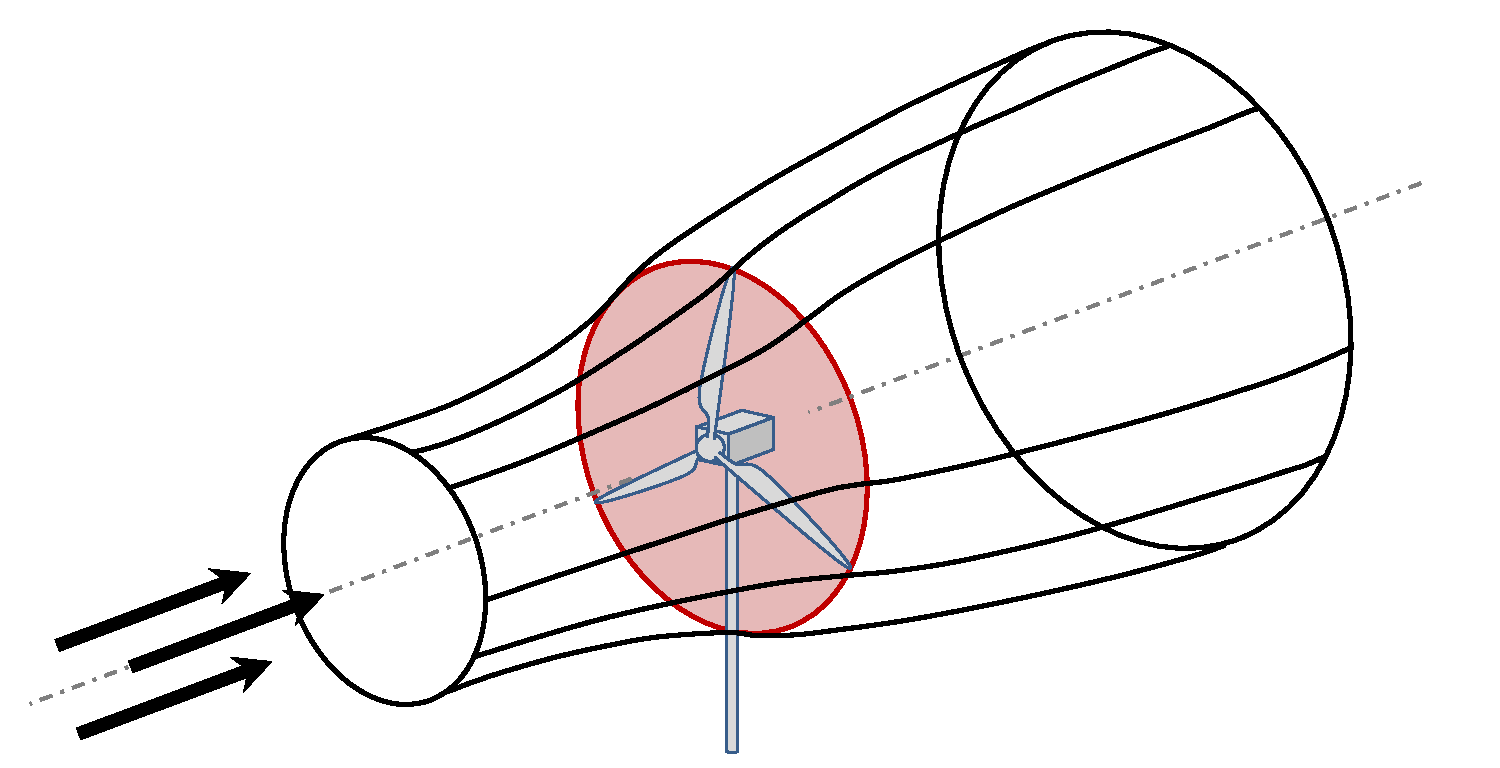
\includegraphics[scale=0.5]{\EPSDIR/Wind_Turbine_fig/Tube.pdf}
\caption{Stream-tube around the rotor disk of a wind turbine. \cite{joulin2019modelisation} adapted from \cite{burton2001wind}}  
\label{fig:BEMTube3D}
\end{figure}		
		
\medbreak
A vertical cut of the stream-tube is given in Figure \ref{fig:BEMTubeEq}. One can write $U$ the axial velocity, $p$ the pressure and $A$ the cross-sectional area. The indices $_\infty$, $_d$ and $_W$ indicate respectively the upstream, disk and downstream positions. The thrust force $F_T$ writes:
\begin{equation}
\label{eq:FpDef}
F_T = A_d (p_d^+ - p_d^-).
\end{equation}		
\medbreak
\begin{figure}[h]
\centering
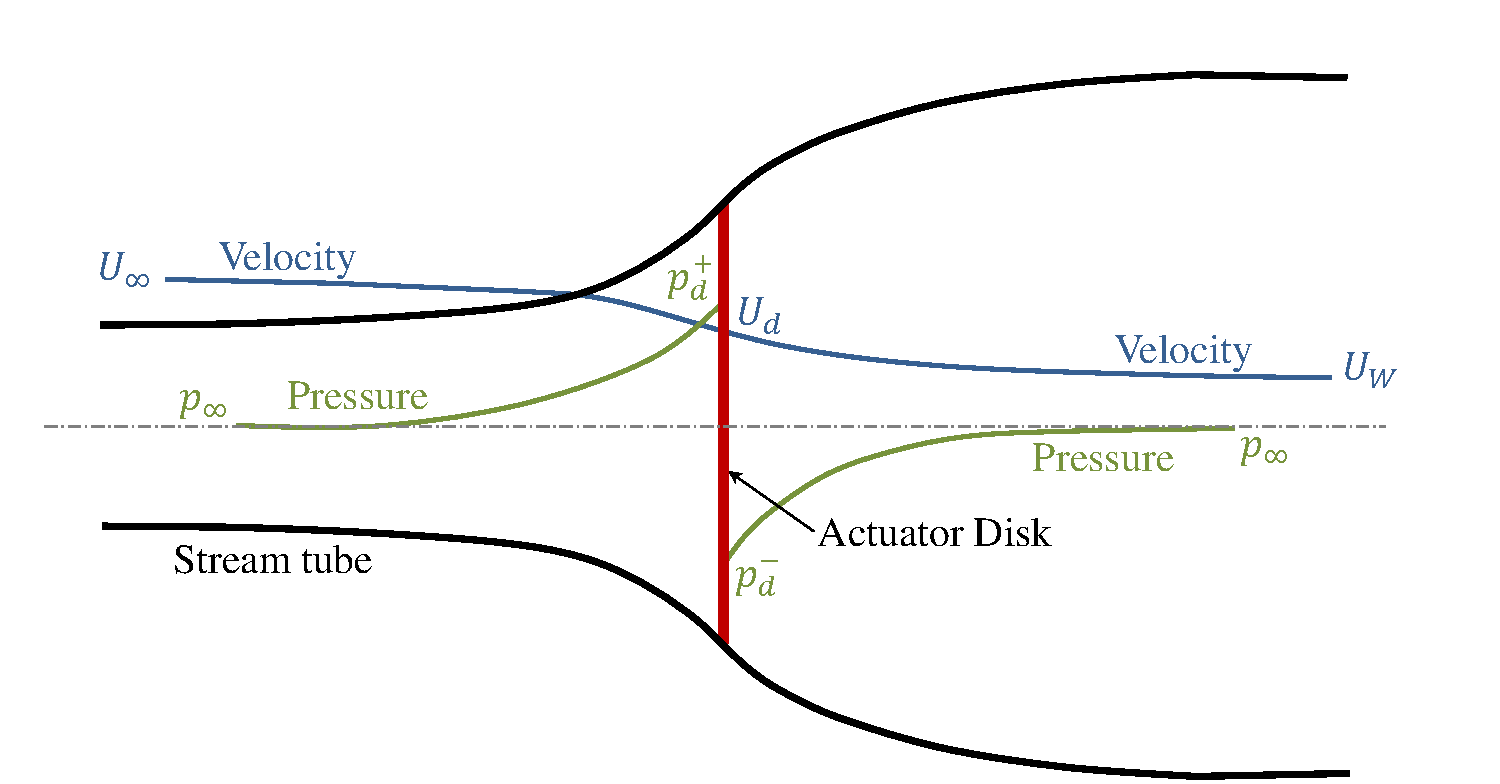
\includegraphics[scale=0.5]{\EPSDIR/Wind_Turbine_fig/Tube_Eq.pdf}
\caption{Vertical cut of the stream-tube around the rotor disk of a wind turbine and its variables. \cite{joulin2019modelisation} adapted from \cite{burton2001wind}}  
\label{fig:BEMTubeEq}
\end{figure}
\medbreak
	
It is possible to apply the Bernoulli’s theorem to the upstream part, and to the downstream one, separately. It gives: 
\begin{equation}
\label{eq:Bern}
\left\lbrace
\begin{array}{ccc}		
p_\infty + \dfrac{1}{2} \rho U_\infty^2 = p_d^+ + \dfrac{1}{2} \rho U_d^2
\\
p_d^- + \dfrac{1}{2} \rho U_d^2 = p_\infty+ + \dfrac{1}{2} \rho U_W^2,
\\
\end{array}\right.
\end{equation}
where $\rho$ is the air density. Using (\ref{eq:Bern}) in (\ref{eq:FpDef}), the thrust force becomes :
\begin{equation}
\fbox{$
F_T = \dfrac{1}{2} \rho A_d (U_\infty^2 -  U_W^2)
$}.
\label{eq:FpBern}
\end{equation}		

This first expression gives the thrust force by knowing the upstream velocity: $F_T = f(U_\infty)$. In practice, it is impossible to define a proper $U_\infty$. Then, an expression with the velocity at the disk position: $F_T = f(U_d)$ has to be found. It is the aim of the next paragraphs.



		\subsubsection*{Momentum theory}
				\label{p:ADNRAppliTheo}

According to the momentum theory applied to a fluid system, the variation of momentum $q$  during $dt$ is equal to the sum of the forces applied on the system. Here, the fluid system is the wind, and the only force applied by the wind turbine against the wind is $F_{T_{WT\rightarrow WIND}}$: 
\begin{equation}
F_{T_{WT\rightarrow WIND}} = \dfrac{d q}{dt}.
\end{equation} 

For a fluid system with a mass $m$, a mass flow rate $D_m$ with an upstream velocity $U_\infty$ and a downstream velocity $U_W$, the variation of momentum can be expressed as:
\begin{equation}
\dfrac{d q}{dt} = D_m (U_W - U_\infty).
\end{equation} 
\medbreak
As it is the thrust force of the wind turbine which is considered: $F_T = F_{T_{WIND\rightarrow WT}}$, it leads to:
\begin{equation}
F_T = D_m (U_\infty - U_W).
\label{eq:FpQm}
\end{equation} 

\bigbreak
According to the stationary hypothesis, the mass flow rate is constant in the stream-tube. By writing its expression at $d$ ($D_m = U_d A_d \rho$), and by using (\ref{eq:FpBern}) and (\ref{eq:FpQm}), one can find:
\begin{equation}
\fbox{$	
U_d = \dfrac{(U_\infty +  U_W)}{2} 
\label{eq:UD}
$}.
\end{equation}

		\subsubsection*{Axial induction factor and thrust coefficient}			
				\label{p:BEMQMFacIndAx}
The axial induction factor $a$ describes the percentage of velocity deficit:
\begin{equation}
U_d = U_\infty( 1 - a ).
\label{eq:a}
\end{equation}
Besides, using (\ref{eq:UD}) et (\ref{eq:a}):
\begin{equation}	
\label{eq:BEMUw}
U_W = U_\infty( 1 - 2a ).				
\end{equation}			
It is now possible to express $F_T$ by using (\ref{eq:FpBern}): 
\begin{equation}	
\label{eq:Fpinf}	
F_T = \dfrac{1}{2} \rho A_d U_\infty^2 4 a (1-a),
\end{equation}
which can be evaluated at disk position thanks to (\ref{eq:UD}): 	
\begin{equation}	
\label{eq:FpD}	
\fbox{$
F_T = \dfrac{1}{2} \rho A_d U_d^2 \dfrac{4a}{1-a}.
$}			
\end{equation}

\medbreak			
The thrust coefficient $C_{T_\infty}$ is the rate between the thrust force and the dynamic force of the wind. One can note that it is defined with the upstream velocity $U_\infty$. It can be expressed using the axial induction factor $a$:
\begin{equation}	
\label{eq:ct}	
C_{T_\infty} = \dfrac{F_T}{\dfrac{1}{2} \rho A_d U_\infty^2} = 4 a (1 -a).
\end{equation}	

		\subsubsection*{Final expression of thrust force}

The thrust coefficient $C_{T_\infty}$  is a well-known data (tabulated data $C_{T_\infty} = f(U_{\infty})$ given by the constructor). Then, by using  (\ref{eq:ct}), one can write $a$ as:
\begin{equation}
a = \dfrac{1}{2}(1-\sqrt{1-C_{T_\infty}}).
\end{equation}
Then, one can define $C_{T_d}$:
\begin{equation}	
C_{T_d} = \dfrac{4a}{1 -a},
\end{equation}	
to finally obtain a suitable expression for the thrust coefficient, using $U_d$ only:
\begin{equation}
\fbox{$
F_T = \dfrac{1}{2} \rho A_d U_d^2 C_{T_d}.
$}		
\label{eq:finadnr}
\end{equation}  

%++++++++++++++++++++++++++++++++
\subsection{Numerical implementation}
%++++++++++++++++++++++++++++++++

In Meso-NH, the ADNR is discretised according to the mesh, as illustrated in Fig. \ref{fig:adnum}.
\begin{figure}[h]
\centering
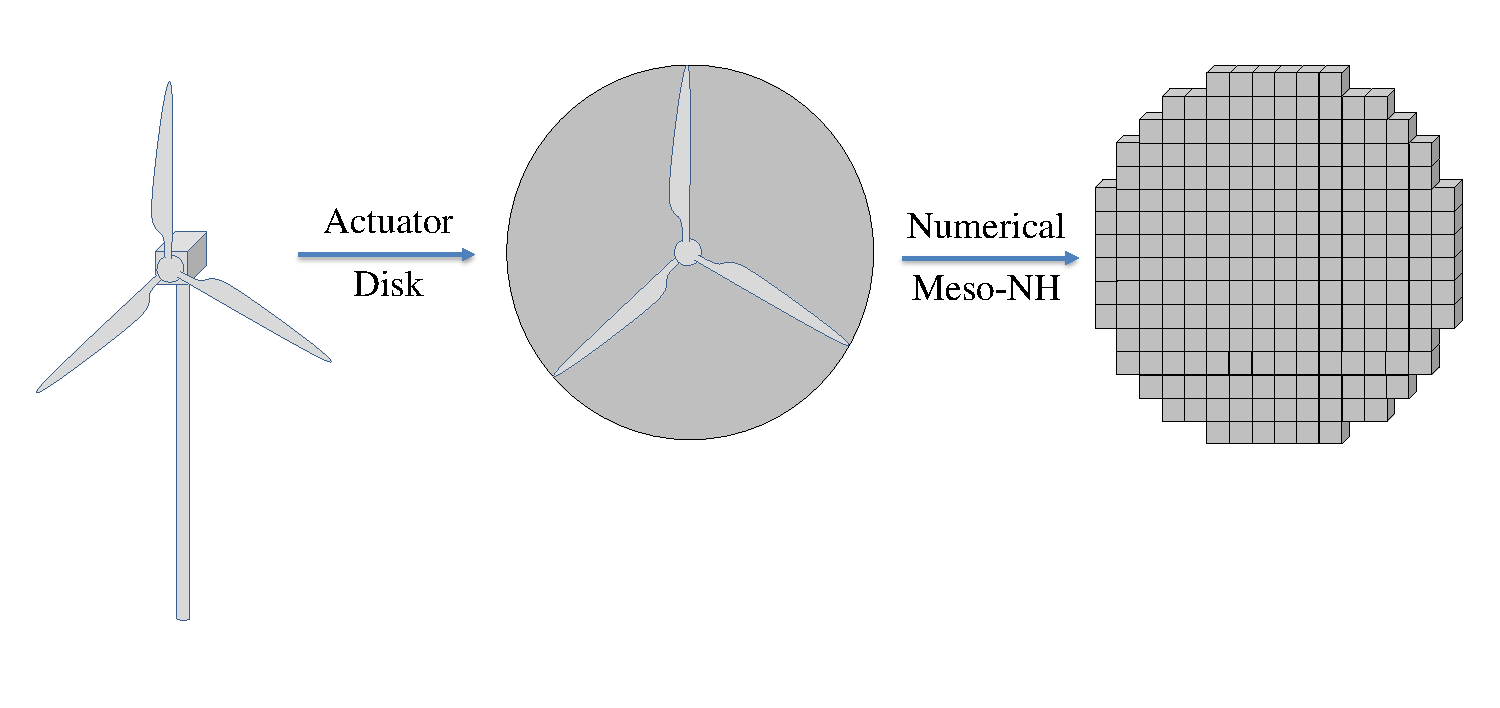
\includegraphics[scale=0.5]{\EPSDIR/Wind_Turbine_fig/ADnum.pdf}
\caption{Discretization of the ADNR \citep{joulin2019modelisation}.}
\label{fig:adnum}  
\end{figure}
\medbreak
The first step of the coupling algorithm is to find the cells where the infinitesimal thrust forces will be applied. It is done by checking if the cell is located into the rotor disk. Then, the wind speed of the cell $U_d$ is extracted, after it has been evaluated at mass point (C-type of Arakawa). It is possible to use the closest value of the wind, or to interpolate it from the 8-neighborhood cells. Finally, the discrete thrust force is calculated by using (\ref{eq:finadnr}) as follows:
\begin{equation}
\fbox{$
dF_T = \dfrac{1}{2} \rho \Delta y \Delta z U_d^2 C_{T_d},
$}	
\label{eq:adnrft}
\end{equation}
where $\Delta y \Delta z$ is the vertical area of the cell. This force will act against the wind field, as shown in Figure \ref{fig:appluforceadnr}. This is why, in the end, the force $dF_{T_{WT\rightarrow WIND}} = -dF_T$ is added to the global momentum budget of Meso-NH. 
\begin{figure}[h]
\centering
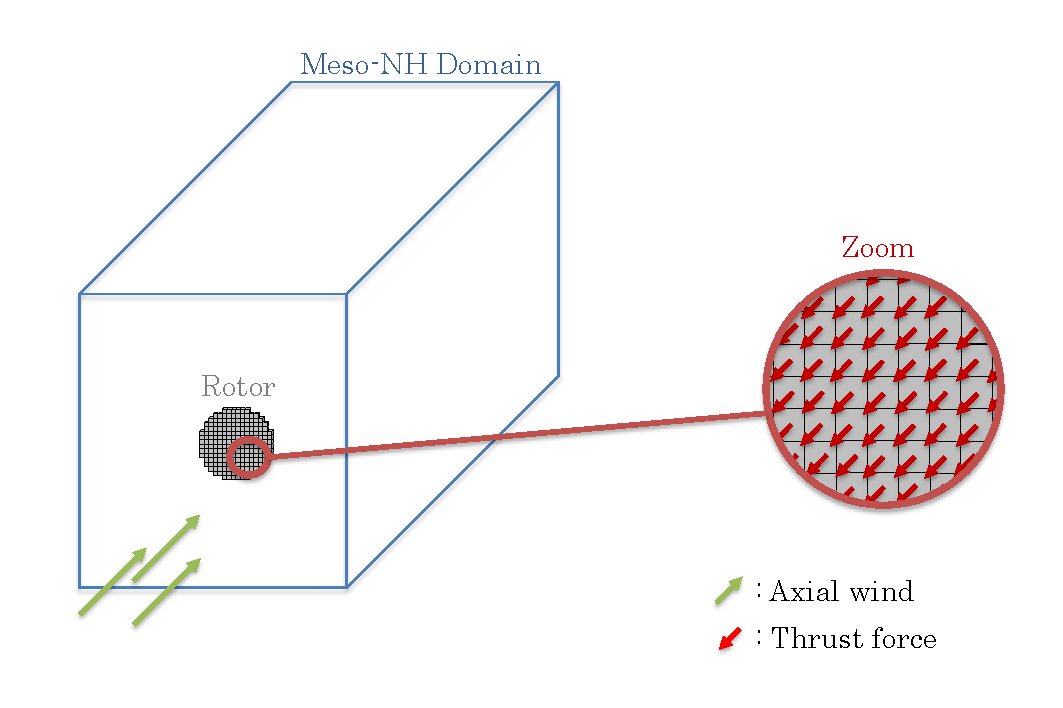
\includegraphics[scale=0.6]{\EPSDIR/Wind_Turbine_fig/ApplyForceADNR.pdf}
\caption{Applying discrete thrust forces in Meso-NH \citep{joulin2019modelisation}.}
\label{fig:appluforceadnr}  
\end{figure}

%++++++++++++++++++++++++++++++++
\subsection{Additional implementations}
%++++++++++++++++++++++++++++++++		
\subsubsection*{1D Linear smearing}
\label{sss:1dsmearADNR}
To avoid numerical instabilities, it is possible to apply a linear smearing to the force field. It is done by using the C-type cells of Arakawa. To smear the forces linearly, one can apply successively:
\begin{equation}
dF_{x_{i}^m} = \dfrac{dF_{x_{i}^f} + dF_{x_{i+1}^f}}{2},
\end{equation}
and then,
\begin{equation}
dF_{x_{i}^f} = \dfrac{dF_{x_{i}^m} + dF_{x_{i+1}^m}}{2},
\end{equation}
where $x_i^m$ and $x_i^f$ are respectively  the mass point and the flux point of the $i^{th}$ cell of $x$-axis. An illustration is given in Figure \ref{fig:smearinglin}. This method is less expensive numerically than the usual convolution product, and seems to provide similar results. See \cite{joulin2019modelisation} for discussions.

\begin{figure}[h]
\centering
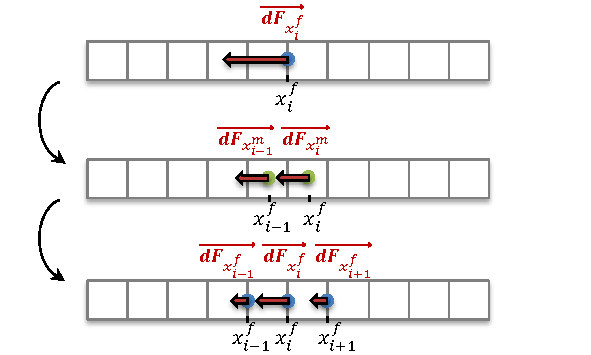
\includegraphics[scale=1]{\EPSDIR/Wind_Turbine_fig/Smearing_Linear.pdf}
\caption{Scheme of an 1D linear smearing of the force field \citep{joulin2019modelisation}.}
\label{fig:smearinglin}  
\end{figure}

\subsubsection*{3D linear smearing}
\label{sss:3dsmearADNR}
It is possible to use a 3D linear smearing based on the 1D Linear distribution, by applying the same method on $y$-axis and $z$-axis successively.




%%%%%%%%%%%%%%%%%%%%%%%%%%%%%%%
\section{Actuator Line Method (ALM)}
%%%%%%%%%%%%%%%%%%%%%%%%%%%%%%%
%++++++++++++++++++++++++++++++++
\subsection{Overview}
%++++++++++++++++++++++++++++++++

The previous model, the ADNR, can be seen as the average of the blade motion over one or several rotations. It gives the tendency of the wake, but it cannot represent its instantaneous particularities. To overcome this problem, it is possible to use lines to model the blades, instead of a disk: it is the \textit{Actuator Line Method} (ALM). The method has been generalized by \cite{sorensen2002numerical}. Each blade applies a force on the fluid, as shown in Figure \ref{fig:AL_principe}. In order to find the position of the blades and their velocity, it is necessary to take into account their kinematic motion. Then, the blade element theory allows to determine the aerodynamic forces to apply.

\begin{figure}[h]
\centering
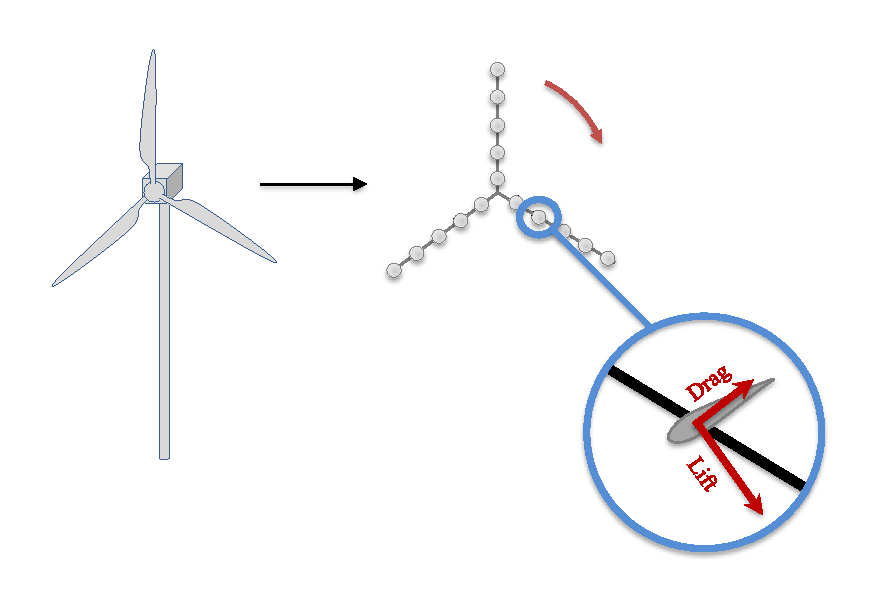
\includegraphics[scale=1]{\EPSDIR/Wind_Turbine_fig/ALprincipe.pdf}
\caption{Overview of the Actuator Line Method \citep{joulin2019modelisation}.}  
\label{fig:AL_principe}
\end{figure}
\medbreak
The first coupling between the Actuator Line Method and a CFD code has been introduced by \cite{mikkelsen2003actuator}. It allows to reproduce the helical shape of the unsteady wake and capturing tip and root vortices (\citep{ivanell2007numerical}, \citep{ivanell2007numericalv}) giving a better description of the wake downstream the wind turbines (\cite{Ivanell2009}, \cite{Troldborg2009}).
\medbreak
For these reasons, the ALM has been introduced in several LES frameworks (\cite{porte2011large} or \cite{tabib2017near}). Interactions between wind turbines and atmospheric boundary layer have been studied (\cite{lu2011large}, \cite{lu2015impact}). It has also been coupled with WRF-LES (\cite{marjanovic2015simulation} and \cite{marjanovic2017implementation}) for wind farm studies, or in SOWFA, based on OpenFOAM  \citep{Churchfield2012}. The coupling with Meso-NH has been introduced by \cite{joulin2020theactuator}.


%++++++++++++++++++++++++++++++++
\subsection{Theory}
%++++++++++++++++++++++++++++++++
\subsection{Hypotheses}
\label{ss:hypALM}
The flow is considered incompressible and 2D along the airfoils.

\subsection*{Wind turbine kinematics and frames}		
\label{ss:EOL_M_cinematiqueAL}

The wind turbine can be divided into different kinematic classes. As shown in Figure \ref{fig:ALrep}, each class has its own frame:
\begin{multicols}{2}
\begin{itemize}
\item the domain associated with $R_G$ frame,
\item the tower associated with $R_T$ frame,
\item the nacelle associated with $R_N$ frame,
\item the hub associated with $R_H$ frame,
\item the $i^{th}$ blade associated with $R_{B_i}$ frames,
\item the $j^{th}$ elements of the $i^{th}$ blade associated with $R_{E_{ij}}$ frames.
\end{itemize}
\end{multicols}
\medbreak
Even if there is no motion between the blade elements and their blade, the frames $R_{E_{ij}}$ linked to the sections have been introduced to make the aerodynamic calculations easier. The rotation matrices $\mathcal{M}_{R_\clubsuit \rightarrow R_\spadesuit}$ are determined at each time step to move from a frame to another one. The kinematic relations allow to know the translational and rotational velocities of each blade element. Details about these relations can be found in \cite{joulin2019modelisation}, \textit{Annexe C}.
\medbreak
\begin{figure}[h]
\hspace{-1.8cm}
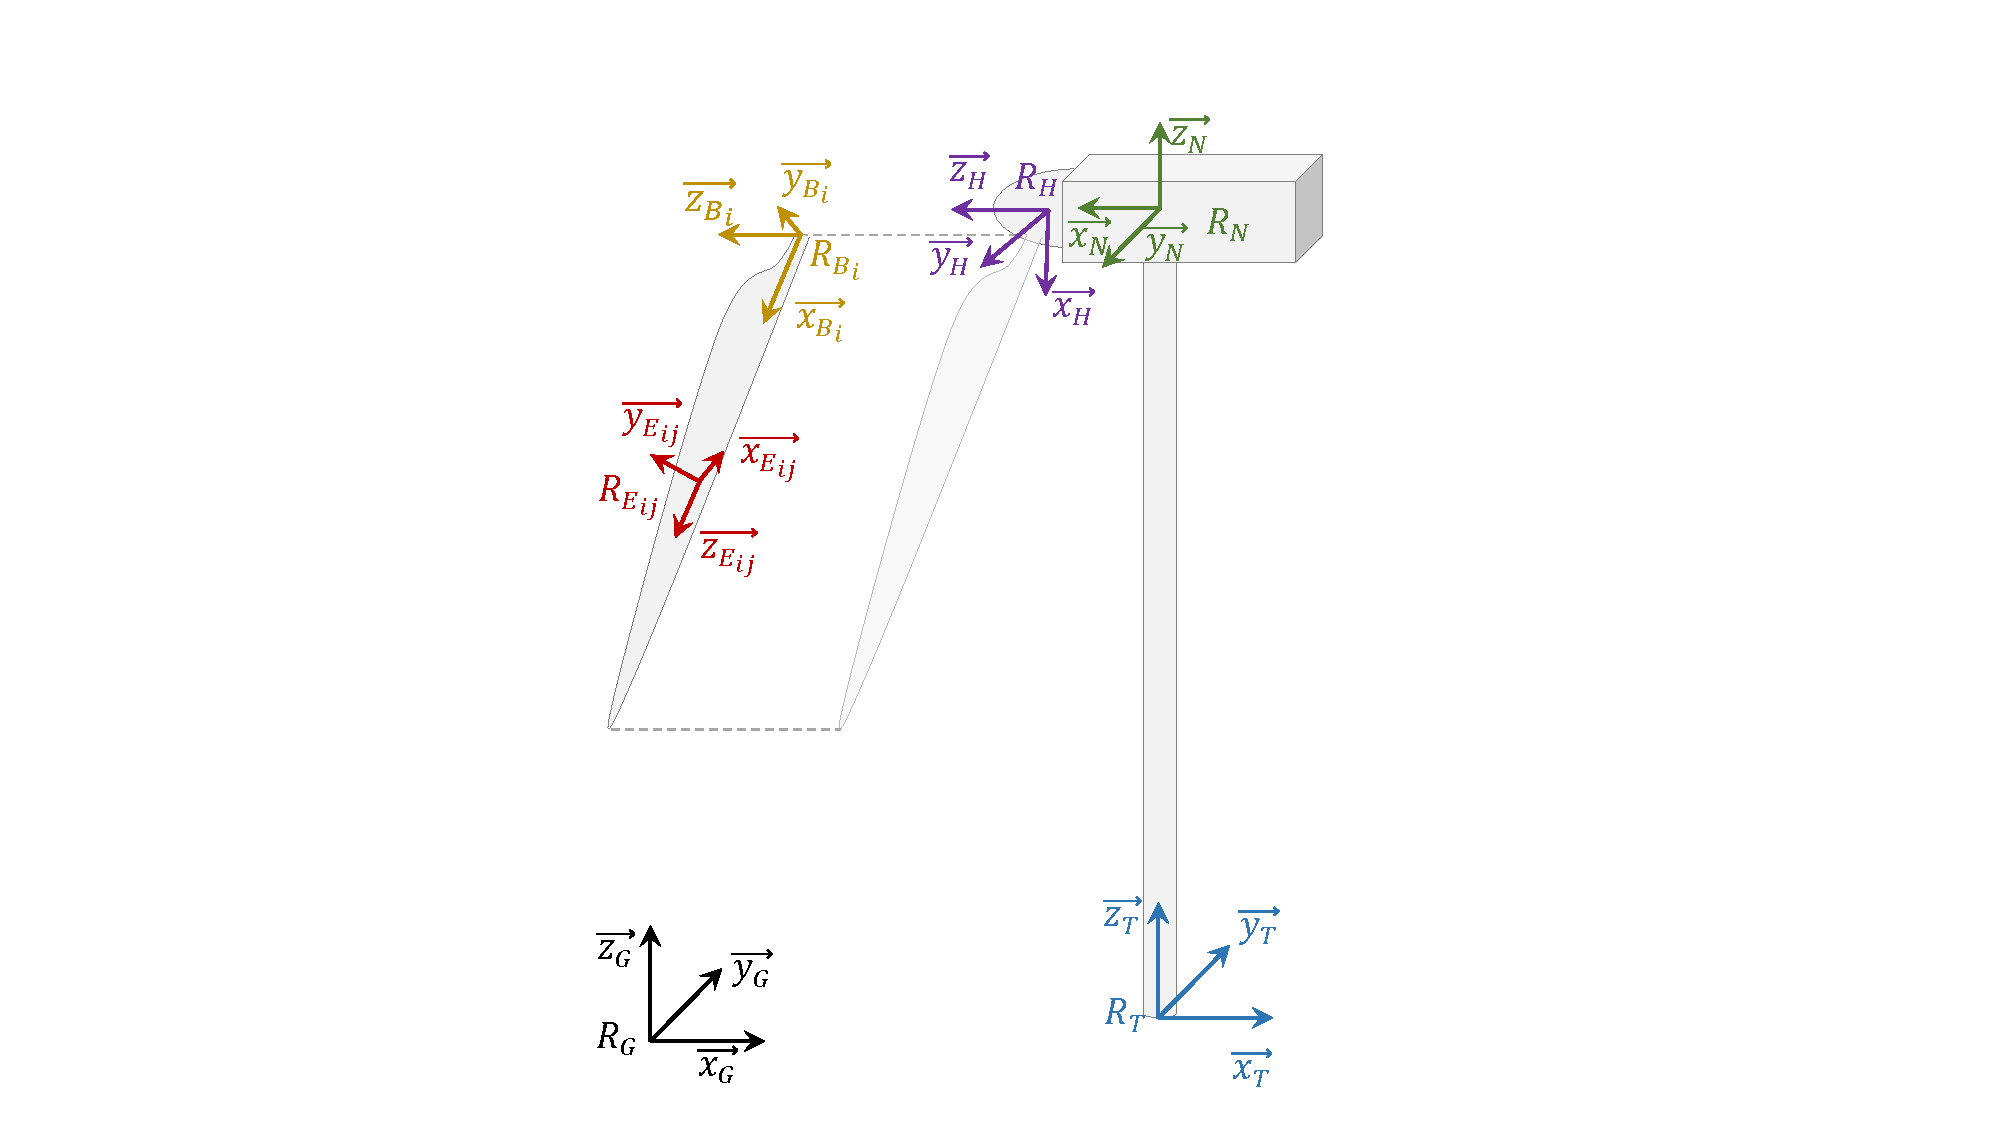
\includegraphics[scale=0.6]{\EPSDIR/Wind_Turbine_fig/CinematiqueRep.pdf}
\caption{Illustration of the frames \cite{joulin2019modelisation}}  
\label{fig:ALrep}
\end{figure}

\subsection*{Applying blade element theory}
										

\subsubsection*{Determination of $U_{rel}$ and $\alpha$}
Thanks to the kinematic definition and to the rotation matrices, the determination of the relative wind $U_{rel}$ is almost direct. Indeed, the kinematic relations enable to know the velocity of translation $U^{ij}_{trans}$. Considering the $j^{th}$ elements of the $i^{th}$ blade located in a surrounding volume of air with a velocity $U^{ij}_{wind}$, the relative velocity writes:
\begin{equation}
\label{eq:AL_urel}
\fbox{$
\overrightarrow{U^{ij}_{rel}}_{\vert _{R_{E_{ij}}}} = \mathcal{M}_{R_{E_{ij}} \rightarrow R_{G_{ij}}} \times \overrightarrow{U^{ij}_{wind}}_{\vert _{R_{G_{ij}}}} - \overrightarrow{U^{ij}_{trans}}_{\vert _{R_{E_{ij}}}}
$}.
\end{equation}
And the angle of attack $\alpha$ can be evaluated thanks to:
\begin{equation}
\label{eq:AL_alpha}
\fbox{$
\alpha = tan^{-1} \left( \dfrac{\overrightarrow{U^{ij}_{rel}}_{\vert _{R_{E_{ij}}}} \cdot \overrightarrow{x}}{\overrightarrow{U^{ij}_{rel}}_{\vert _{R_{E_{ij}}}} \cdot \overrightarrow{y}} \right)
$}.
\end{equation}

\subsection*{Aerodynamic forces}
By knowing $U_{rel}$ and $\alpha$, the blade element theory can be applied. The aerodynamic forces can be expressed in the aerodynamic frame as:
\begin{equation}
\label{eq:eol_m_alm_eff}	
\fbox{$
\left\lbrace
\begin{array}{ccc}	
dF_{L} = \dfrac{1}{2} \rho S U_{rel}^2 C_L,
\\   
\\
dF_{D} = \dfrac{1}{2} \rho S U_{rel}^2 C_D.
\\
\end{array}\right.
$}
\end{equation}	

where the lift $C_L$ and drag $C_D$ are known according to the angle of attack $\alpha$ and the Reynolds number $Re$. The lifting surface $S$, evaluated with the airfoil chord $c$ and the radial width $dr$ ($S = c dr$). By applying a rotation angle $a$, the forces can be expressed in $R_{E_{ij}}$, and then in the global frame by using $\mathcal{M}_{R_{G_{ij}} \rightarrow R_{E_{ij}}}$.

%++++++++++++++++++++++++++++++++
\subsection{Numerical implementation}
%++++++++++++++++++++++++++++++++

The first step of the Actuator Line Method algorithm is to compute the kinematics of the wind turbine. An illustration of the kinematic classes and their discretization is shown in Figure \ref{fig:ALMdiscret}. The kinematic algorithm computes, at each time step, the new positions and velocities of all elements. 
Knowing the position of a blade element, the local wind speed can be extracted. To do so, the wind speed is computed at mass point. Then, it is possible to use the closest value (from the blade element) of the wind, or to interpolate it from the 8-neighborhood cells.
Afterwards, the relative velocity is computed using (\ref{eq:AL_urel}), and the angle of attack $\alpha$ with (\ref{eq:AL_alpha}). The aerodynamic coefficients $C_L$ and $C_D$ are then computed by knowing $\alpha$, from a spline-cubic interpolation of the tabulated input data. Finally, the aerodynamic forces are computed in the aerodynamic frame using (\ref{eq:eol_m_alm_eff}): 
\begin{equation}
\label{eq:eol_m_alm_eff_num}	
\fbox{$
\left\lbrace
\begin{array}{ccc}	
dF_{L} = \dfrac{1}{2} \rho c \Delta r U_{rel}^2 C_L(Re,\alpha),
\\   
\\
dF_{D} = \dfrac{1}{2} \rho c \Delta r U_{rel}^2 C_D(Re,\alpha).
\\
\end{array}\right.
$}
\end{equation}	
A last change of frame enables the projection of these forces to the global momentum budget of Meso-NH. One can note that, for the moment, only the effects of the blades are computed: the nacelle and the tower are neglected. 
\begin{figure}[h]
\centering
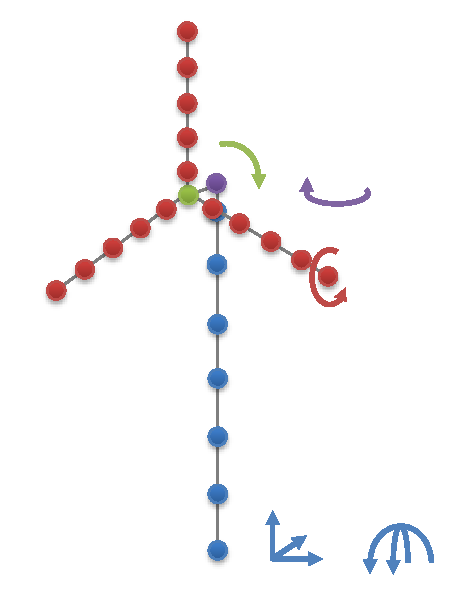
\includegraphics[scale=0.8]{\EPSDIR/Wind_Turbine_fig/ALdiscret.pdf}
\caption{Illustration of the discretised kinematic classes of the ALM. Each color is a different class, and each arrow indicates a possible motion. \cite{joulin2019modelisation}}
\label{fig:ALMdiscret}  
\end{figure}


%++++++++++++++++++++++++++++++++
\subsection{Additional implementations}
%++++++++++++++++++++++++++++++++
\subsubsection*{1D linear smearing}
It is possible to use the 1D linear smearing mentionned in \ref{sss:1dsmearADNR}.

\subsubsection*{3D linear smearing}
It is possible to use the 3D linear smearing mentionned in \ref{sss:3dsmearADNR}.

\subsubsection*{Tip loss correction}
\label{sss:tiplossALM}

An over-estimation of loads is commonly predicted by the Actuator Line Method. It appears when the mollification (smearing) or the resolution are not adequate to generate de tip vortices and so the tip losses. 
To overcome this issue, the community usually applies the tip loss correction of \cite{glauert1935airplane}, showing a better prediction of the loads (\cite{mikkelsen2003actuator} or \cite{shen2005tip}). This correction was initially introduced to correct BEM-like models (such as  Rotating Actuator Disk), where an infinite number of blade is considered. \cite{glauert1935airplane} introduced a factor $F$ to take into account the wake induced losses:
\begin{equation}
F = \dfrac{2}{\pi} \arccos( e^{-f})
\end{equation}
where $f$ can be expressed using the radius of the tip $r_{tip}$, the radius of the hub $r_{hub}$ and the flow angle $\varphi$:
\begin{equation}
f=
\left\lbrace
\begin{array}{cc}
\dfrac{N_{pales}}{2} \dfrac{r_{tip}-r}{r sin(\varphi)}  & \mbox{for blade's tip,}\\
\dfrac{N_{pales}}{2} \dfrac{r-r_{hub}}{r sin(\varphi)}  & \mbox{for blade's root.} 
\\
\end{array}\right.
\end{equation}
Then, the factor is introduced as follows:
\begin{equation}	
\label{eq:ADR_tiploss}
\left\lbrace
\begin{array}{ccc}	
dF_{L} = \dfrac{1}{2} C_L \rho S U_{rel}^2 F,
\\   
\\
dF_{D} = \dfrac{1}{2} C_D \rho S U_{rel}^2 F.
\\
\end{array}\right.
\end{equation}	
One can note that in the ALM, the number of blade is finite and this correction should not be used. Some specific corrections could be implemented, as shown by \cite{breton2008study}. Besides, a better distribution of forces is also possible as proposed by \cite{churchfield2017advanced}. 
As Meso-NH is a meteorological tool, the resolution might be too large compared to the guidelines recommanded for the ALM \citep{jha2014guidelines}. Then, the tip loss correction is applied by default in Meso-NH (LTISLOSSG = .TRUE.).

\subsubsection*{Time-splitting method}
\label{sss:time_splitting}
In order to save computational cost, a time-splitting method has been introduced \citep{joulin2020theactuator}. This method is also called Actuator Sector Method \citep{Storey2015}. 
The Courant-Friedrichs-Lewy (CFL) criterion of Meso-NH imposes a time step $\Delta t_{MNH}$. The criterion writes:
\begin{equation}	
n_{CFL} =  c \dfrac{\Delta t_{MNH}}{min(\Delta x,\Delta y,\Delta z)},
\label{eq:MNH_CLF}
\end{equation}  
where $c$ is the flow velocity, and  $\Delta x$, $\Delta y$, $\Delta z$ the cell sizes. In Meso-NH, $n_{CFL} < 3$ is imposed according to the scheme used.
\medbreak
Nevertheless, the ALM often requires a smaller time step in order to ensure that a blade element point will not skip a mesh cell during this time step. The criterion for the Actuator Line Method time step $ \Delta t_{ALM}$ can thus be expressed as:
\begin{equation}
\Delta t_{ALM} \leqslant \dfrac{min(\Delta x,\Delta y,\Delta z)}{\Omega r_{tip}},
\label{eq:dt_alm}
\end{equation}
where $\Omega$ is the angular velocity of the wind turbine, and $r_{tip}$ the tip radius of the blade.
\medbreak
Because Meso-NH does not need such a small time step, a $\Delta t_{MNH}$ respecting the CFL criterion is preserved. On the other side, the ALM algorithm is called $N_{split}$ times over this duration in order to respect the ALM time step criterion (eq. (\ref{eq:dt_alm})) and to reduce by $N_{split} - 1$ the number of iterations from the LES solver.
\medbreak
\begin{figure}[h]
\centering
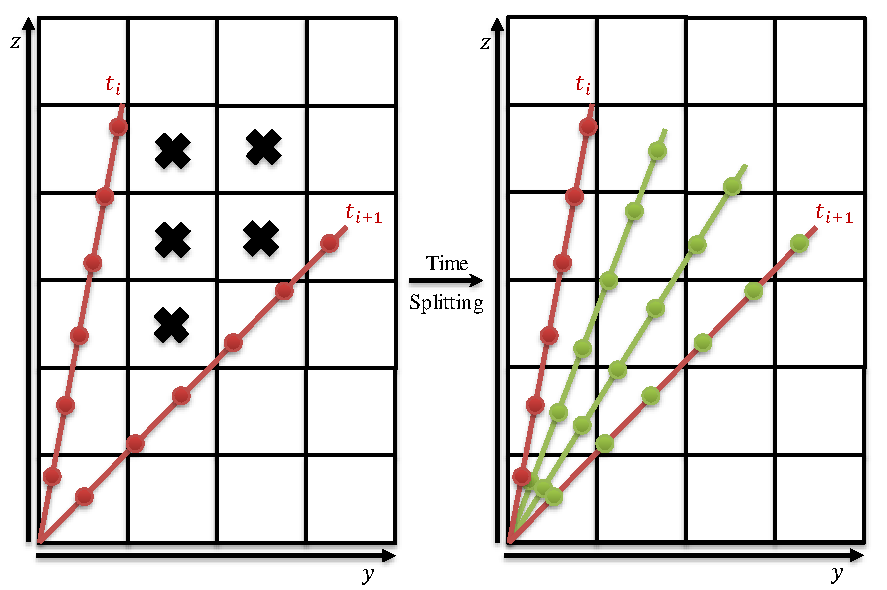
\includegraphics[scale=0.8]{\EPSDIR/Wind_Turbine_fig/Time_Splitting.pdf}
\caption{Illustration of time-splitting method, for $N_{split} = 3$. \cite{joulin2019modelisation}}
\label{fig:timesplit}  
\end{figure}
The method is illustrated in Figure \ref{fig:timesplit}. The red lines indicate blade positions at $t_{i}$ and $t_{i+1}$. The red dots indicate blade elements. The black crosses on the left Figure show the cells missing the blade passage. On the right, the time-splitting method enables to get the history of the blade motion (green lines and dots) to compute to aerodynamic forces.

One can note that during a Meso-NH time step, the wind field is frozen. In the end, for each blade element point, the applied force is the aerodynamic force evaluated by the ALM divided by $N_{split}$ to respect the momentum budget over $\Delta t_{MNH}$.


%%%%%%%%%%%%%%%%%%%%%%%%%%%% BIBLIOGRAPHY %%%%%%%%%%%%%%%%%%%%%%%%
\begin{btSect}{3-10-WindTurbine}
\section{References}
\btPrintCited
\end{btSect}
%%%%%%%%%%%%%%%%%%%%%%%%%%%% BIBLIOGRAPHY %%%%%%%%%%%%%%%%%%%%%%%%
